\chapter{绪论}

\begin{figure*}
\center{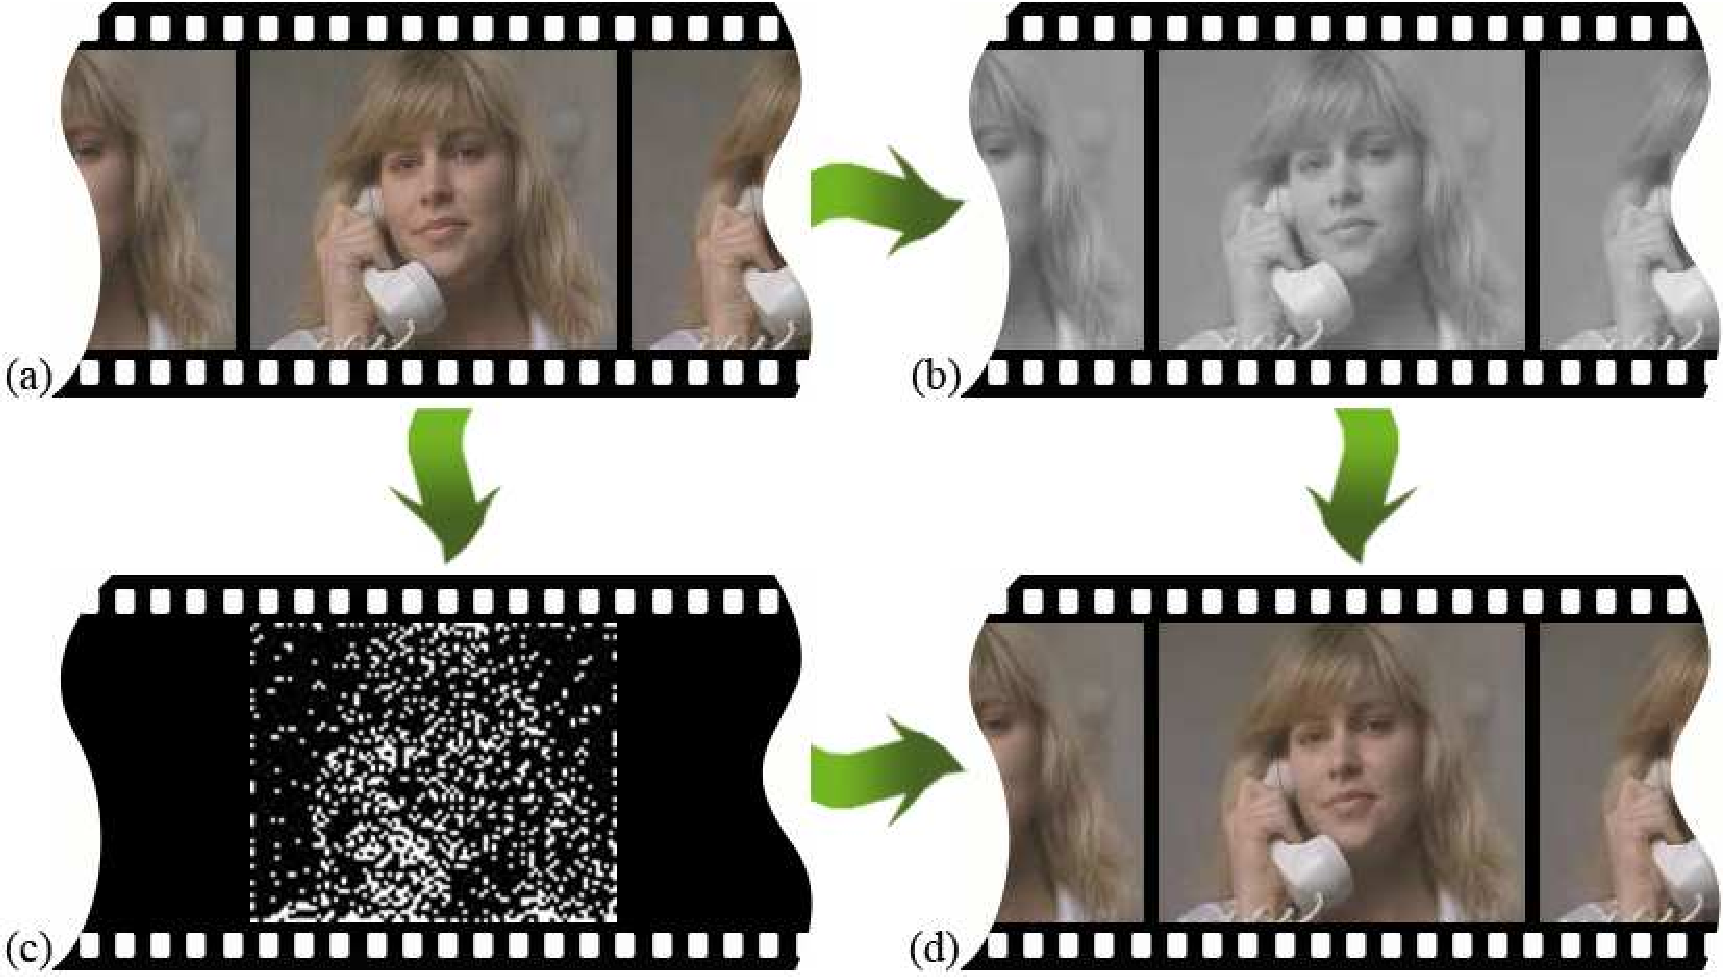
\includegraphics[width=380pt]{images/cycle}}
\caption{\label{fig:cycle}基于学习的视频压缩的例子。 (a) 原始视频帧
(b) 灰度帧 (c) 选取的带有颜色信息的点 (d) 恢复的视频帧}
\end{figure*}

随着计算机技术的进步和互联网的飞速发展,数字视频不管从数量还是从复杂度上都呈现出爆炸性的增长。
视频压缩是一项用于缓解视频存储空间以及传输带宽占用的关键性技术。视频数据通常包含了许多时间和
空间上的冗余信息。相似信息可以通过编码帧内(空间上的)或帧间(时间上的)差异的方式来进行存储。
典型的压缩方法包括了离散余弦变换、向量化、分形压缩以及离散小波变换等。

最近 \cite{learning-to-compress-images}
提出了基于机器学习的视频压缩方法。他们提出了和传统的频域转换不同的方式,将原始的带颜色的视频
转化为一个灰度视频,选取一些有代表性的点并存储他们的颜色信息,然后使用灰度视频和带有颜色信息
的点学习出一个统计模型,用于预测其他像素点的颜色值。实验结果表明,在保证图像质量(通过
PSNR
\footnote{http://en.wikipedia.org/wiki/PSNR}进行衡量)的前提下,可以达到不错的压缩效果。

从机器学习的视角来看,这里主要有两个基本的问题。首先是如何选取最有代表性的点,这本质上是一个
主动学习(Active
Learning)的问题。存储灰度视频和选出来的颜色点的信息就是编码的过程。
其次是如何结合选出来的带颜色信息的点和灰度视频来学习一个模型,这在本质上是
一个半监督学习(Semi-supervised
Learning)的问题。用这个模型来恢复原始视频就是解码的过程。在这里有颜色的像素被当作是带标签的
数据,而灰度像素则被当作是无标签的数据。\cite{learning-to-compress-images}
使用了一种非常直接的主动学习的方法:在每一次迭代的时候简单地在预测错误率最高的区域选点。在选
点之后他们使用拉普拉斯正则化的最小二乘法(LapRLS,\cite{Manifold-Regularization-Journal})来
完成半监督学习的问题。他们的方法的最大的不足就是没有任何理论上的依据可以保证使用这种方法选出来
的点可以降低预测的错误率。

在本文中,我们提出一个针对视频压缩的自主学习和半监督学习的统一框架。我们的方法的中心思想是颜色
点的选取和后续的着色过程应该同时进行优化。具体来讲,对于着色的过程,我们假定每个像素的颜色值可以
通过其(时间或空间上的)邻居中灰度值相似的像素的颜色值重新构造出来,并使用正则化的最小二乘法
来学习一个模型;对于选点的过程,我们使用相同的损失函数(loss
function),并使用最小化系数的协方差矩阵的准则来进行选点。然后我们还讨论了如何将自主学习和半监督
学习结合起来应用到视频压缩上面。学习出来的模型不仅用于预测当前的帧,而且还被用于预测后续的相似的
帧,知道 PSNR 分值降低超过了一定的阈值,再重新训练一个模型。图
\ref{fig:cycle} 展示了我们的方法是如何工作的。

论文余下的部分是这样组织的:在第二章中,我们简要地回顾了一下这个领域相关的工作。用于着色的半监督
学习的办法将会在第三章中介绍。第四章介绍如何通过主动学习选取最具代表性的点。然后我们会在第五章中
给出一个用于食品压缩的主动学习和半监督学习的统一框架。实验结果将在第六章中展示。第七章我们将会进行
简要总结并展望后续的工作。

